\documentclass[fontsize=11pt]{article}
\usepackage{amsmath}
\usepackage{graphicx} 
\usepackage[utf8]{inputenc}
\usepackage[margin=0.75in]{geometry}

\title{CSC110 Final Project: \\ Investigating the Implications of $CO_2$ Levels on the Number of Forest Fires in the US}
\author{Group Members: Leya Abubaker, Armaan  Mann, Ansh Malhotra, Gabriel Pais}
\date{Monday, December 14, 2020}

\begin{document}
\maketitle
\section{Introduction}
\subsection{Problem Description and Research Question}

\textbf{Research Question:
Is there a correlation between CO2 Emissions and the Frequency of Wildfires in the US?}


Greenhouse gases are gases that trap heat inside the Earth's atmosphere. Carbon Dioxide makes up most of the greenhouse gas emissions in our world and is emitted through the burning of fossil fuels such as petroleum (“Overview of Greenhouse Gases”, 2020). The United States was ranked second in the world's CO2 emissions, which produced approximately 5,269.5 million metric tons in 2017 (Frohlich and Blossom, 2019). Greenhouse gases, like carbon dioxide, are major factors of global warming because they cause the Earth’s temperature to rise which can lead to an increase in many forms of natural disasters (Osmanski, 2020).  In particular, the hot and dry temperatures cause the vegetation in forests to dry out and it increases the risks of forest fires and the damages that it can cause. Forest fires can also increase the emissions of CO2 in the atmosphere, which continues to increase the global temperature and in turn increases the frequency of extreme weather events (Gray, 2019). \\
\newline
It is important to note that the majority of forest fires are caused by humans, so our project topic seeks to determine whether CO2 emissions have an impact on the frequency of forest fires and how much of an impact it may have. We chose to study the relationship between CO2 emissions and the frequency of wildfires because we noticed that there have been an increase of forest fires reported in the news, especially in the US, and from our research we discovered that the US CO2 emissions are very high. So, we wanted to determine if there is an actual connection between the increase in the occurrences of wildfires in the US, to the amount of CO2 that is emitted. The project topic that we wish to analyze directly relates to climate change because the damage that natural disasters, like forest fires, cause are increased due to global warming. So the focus for our project is to determine whether larger emissions of CO2 specifically correlate to a higher frequency in forest fires. 
\newline 

\textbf{Changes Made from Original}

Based on the feedback provided from the TA we reformulated our question into 
determining if there is a correlation between CO2 emissions and forest fires. To answer this question, instead of plotting a linear regression we decided to plot a bar graph that displays the CO2 emissions of a particular state with a line graph that plots the number of forest fires that occurs each year. We also included a separate graph that displays this information for the United States. From these plots we analyzed the trend between the year with the highest level of CO2 emissions and the year with the highest number of forest fires to check if our hypothesis is correct. In addition, we also changed our final output and computation. Instead of just producing a heat map, we decided to create a map of the US that displays the amount of forest fires that occurred in each area as clusters for one entity with the addition of a heat map. In which each zoom level has more information for a particular location of the forest fire. As well as an interactive portion that shows extra information about the forest fires in that particular state and provides a link to extra information about the forest fires. The heat map allows the user to filter to either the Vegetation, Fire Magnitude, Wind at that time and Humidity at that time as a layer on top of the pre-existing map, to show how various areas of the US are effected.\\
\pagebreak

\subsection{Dataset Description}

\begin{enumerate}
    \item We have used four datasets for this project, we manually created all of them. The first one is the US Wildfire Data (under the name of FireData5yrs.csv), which is used to create the US map and shows the values for each forest fire with its respective data. The dataset has been filtered to just 5 years to maintain performance and ensure that the graph is still interactive, any more than that would fill the map with over 35,000 forest fires and would take a tremendous amount of time to load. This dataset contains the year when the wildfire occurred ( 2010 -  2015), the state where the wildfire happened ( LA, MS, NY…), the fire\_size, fire\_size\_class, the latitude and longitude, vegetation, fire\_mag,  wind\_cont. See legend for details on what each value represents.
    \item The second dataset represents the same Wildfire Data (called FireData10yrs.csv), it contains the same values as the previous dataset (FireData5yrs.csv), except for years. This data set is used to state names and the year from the variables state\_name and Date (Year). We have filtered this data to just 10 years (2005-2015) by removing all empty lines and cutting out almost half of our original dataset.
    \item Our third dataset is a CO2 data set (named CO2\_DataSet.csv). This dataset contains information about each state with the level of CO2 emissions for each year between 2005 and 2015 inclusive. This dataset was also filtered to 10 years from 2005 to 2015.
    \item The last dataset has the name overlay.json and contains coordinates manually taken by us of the US border. The file is used in our mapping to show the border of the United States.  

\end{enumerate}
All these files are csv files except the last one which is a json file.

\noindent\textbf{We got our datasets from the following sources:}
\begin{itemize}
    \item “U.S. Wildfire Data (plus Other Attributes).” Kaggle, 6 Oct. 2020, www.kaggle.com/capcloudcoder/us-wildfire-data-plus-other-attributes.
    \item The source of the CO2 Data is from the following website: https://www.eia.gov/environment/emissions/state/
    \item The source of the coordinates data is from the following website : www.geojson.io
\end{itemize}


\subsection*{Legend:}
\begin{itemize}
    \item Vegetation - Type of Vegetation.
    1:Tropical Evergreen Broadleaf Forest, 2:Tropical Deciduous Broadleaf Forest, 3:Temperate Evergreen Broadleaf Forest ,
4:Temperate Evergreen Needleleaf Forest TmpENF,5:Temperate Deciduous Broadleaf Forest,6:Boreal Evergreen Needleleaf Forest,7:Boreal Deciduous Needleleaf Forest, 8:Savanna , 9:C3 Grassland/Steppe, 10:C4 Grassland/Steppe, 11:Dense Shrubland 12:Open Shrubland, 13:Tundra Tundra, 14:Desert,15:Polar Desert/Rock/Ice, 16:Secondary Tropical Evergreen Broadleaf Forest, 17:Secondary Tropical Deciduous Broadleaf Forest, 18:Secondary Temperate Evergreen Broadleaf Forest, 19:Secondary Temperate Evergreen Needleleaf Forest
20:Secondary Temperate Deciduous Broadleaf Forest, 21:Secondary Boreal Evergreen Needleleaf Forest, 22:Secondary Boreal Deciduous Needleleaf Forest, 23:Water/Rivers Water
24:C3 Cropland, 25:C4 Cropland, 26:C3 Pastureland, 27:C4 Pastureland, 28:Urban land
\item Fire\_size = the size of the fire \item Fire\_size\_class = class of the fire size (A - G)
\item Latitude and Longitude = coordinates of the fire on the map
\item Fire\_mag = the magnitude of fire intensity (scaled version of fire\_size)
\item Wind\_cont = wind in m/s at the location of fire up to the day the fire was contained
\item Hum\_cont = humidity in percent at the location of the fire up to the fire was contained.
\item Remoteness = the distance to the closest city
\item Urls = different links representing information about fires from different states, each state has a different url
\end{itemize}

\pagebreak

\section*{Computational Plan}

To start off, we looked at the datasets called raw\_firedata and raw\_co2\_data. The raw data from the fire dataset was huge with many columns and numerous rows. Due to this, we had to shrink the domain of the years to 5 years and 10 years. The two datasets are used throughout the code for visualizations and graphs. Specifically, the 10 year data set is used for the bar plot with line in plot.py and the 5 years dataset is used for the map.py. Next, to obtain these smaller domain datasets, the raw sets were filtered to 2005 to 2015 and all the empty cells along with the rows they belonged to were removed. Likewise, the same steps were repeated for the other fire dataset but for only 5 years from 2010 - 2015 inclusive. In the file \‘FireData5yrs.csv\’, we removed all the empty cells and respective rows and also added one url for each state manually, and the column names were just filtered to latitude, longitude, fire size, vegetation, fire magnitude, wind contained at that time, humidity contained at that time and remoteness (Same thing was done for \‘FireData10yrs.csv\’ but no urls were manually inputted as that file is used for the line bar plots). \\
\newline
Since all the datasets were stored as csv files, the library \‘import csv\’ was used to extract the data from the excel file. There are 3 functions altogether which collects the data from the csv file and then stores the data into the dictionary, with its keys being the column names, which are as follows: read\_data\_fire (for 10 years from the forest fire dataset), read\_data\_co (for the CO2 data set) and read\_data\_map (for 5 years from the forest dataset). The data wrangling for the forest fires were made in two different files because when creating the map there were too many values which was causing the program to load for too long and eventually crashing chrome and pycharm. Therefore, we decided to shrink the domain to 5 years. All the data wrangling was done in main.py. \\
\newline
Next, our program has two visualizations: one is based on states and another one is generalized to all of the US. To begin, the get\_data\_fire is used to get the number of years from the \‘FireData10yrs.csv\’ using the data wrangling function called read\_file\_fire which also obtains the y-values (fire frequencies gets added per state) which is used for the line graph portion. Also, the function get\_data\_co2 is used to collect the values for the bar graph portion of the plot. The y-values in this case are obtained from the \‘CO2\_DataSet.csv\’ from 2005 to 2015. Finally, we also used a helper function which is used to add all the forest fire frequencies using the \‘FireData10yrs.csv\’. All the functions are also in main.py.\\
\newline
Furthermore, the second file that was created just for the plots is called plots.py. This is the file which contains the major visualization of the line bar plot. The file contains two functions that perform the visualization. The first function, state\_plot, displays a line bar plot that displays the relationship between CO2. emissions of a particular state (chosen by the user) and the number of forest fires in that state. The second function, entire\_plot, displays a line bar graph that shows the relationship of CO2 emissions for the US as a whole and the total number of forest fires occurrences  in the US. These visualizations were created using the plotly library. Specifically, we used the libraries plotly.graph\_objects and plotly.subplots functions to help display our visualizations of the graphs. We decided to use the plotly library because it has more features and is more interactive compared to other libraries. 
The data is then analyzed by the functions check\_trend and check\_trend\_all which returns whether or not the data we collected follows the trend we initially predicted. \\
\newline
For Map.py, the major computations performed were in regard to data wrangling. Firstly, we needed to organize and store the data from ‘FireData5yrs.csv’ in a way that would allow us to place markers on the map according to the wildfire’s latitude and longitude. Therefore, out of the raw dataset, only latitude, longitude, fire size, vegetation, fire magnitude, wind contained at that time, humidity contained at that time and remoteness were stored. A data frame was created to store all these key value pairs to be used in the map which is used by the library called pandas.\\
\newline
Secondly, the os library was used to implement the json file in the visualization. First off, the json file called overlay.json was created through a website that allowed the user to outline a certain area of the world map and then after selecting the area stored the coordinates. Thus after transferring the coordinates to a json file, using the os library we were able to add the outline to the map we created. \\
\newline
Next, the main library that was used to construct the visualization was folium. The following methods were used from the folium library: folium.Map(), folium.plugins.MarkerCluster(), folium.Marker(), folium.GeoJson(), folium.plugin.MiniMap(), folium.Fullscreen(), folium.TileLayer(), folium.LayerControl(), m.save(), folium.Choropleth(). Comments are attached to the code itself for more descriptive uses of the methods mentioned above.  



\pagebreak

\section*{Instructions: main.py and plots.py}
\begin{enumerate}
    \item To begin you need to install the plotly package and the csv package. To do so, start off by opening Pycharm and going to File $\rightarrow$ System $\rightarrow$ Project $\rightarrow$ Python Interpreter, click the add button and type $plotly$ into the search bar and click install to install the package. Do the same for the csv package. 
    \item Next, with the files provided through Markus, download main.py,  plots.py, $FireData10yrs.csv$ and $CO2\_DataSet.csv$ into the same folder. For the raw Fire Data and CO2 Data, check UTSend and download the data if needed(you will not need the raw data to run this file or have any functions that use the raw data) \\
    Claim ID: dUP2g9A9zepxR8ai \\
    Claim Passcode: nBN2Auw8Dt9zNSfN
    \\
    \item Ensure that the folder in which you store all the files in is a source root folder, do not create a sub-folder since it’s not needed.
    \item Import the libraries, check the requirements.txt file for all the libraries and their corresponding versions.
    \item In the main.py python file:
    \begin{itemize}
        \item The functions $read\_file\_co$ and $read\_file\_graph$ are used for data wrangling, it can be called to view the processed data as a dictionary. In order to call the function, $read\_file\_graph$ the user must call the function in the console and pass “$FireData10yrs.csv$” as the argument to view the processed data. In order to call the function, $read\_file\_co$ the user must call the function in the console and pass “$CO2\_DataSet.csv$” as the argument to view the processed data (make sure to include quotations). It includes helper functions to get the points of each plot. The functions $get\_data\_fire$ and $get\_data\_co2$ is used to return the x and y-values for the line and bar graph per state. To call these functions, the user must pass a state name in the form of an abbreviation as a parameter. For example New York - ‘NY’, Florida - ‘FL’. Finally, the helper function $total\_fire$ is used to obtain the y-values of the total number of forest fires in the US. 
    \end{itemize}
    \item In the plots.py python file:
    \begin{itemize}
        \item The function $state\_plot$ is used to display the graph of a particular state. When calling this function the user must pick a state that they would like to see a graph of and pass its abbreviation as a parameter. For example New York - ‘NY’, Florida - ‘FL’.\\
            \begin{figure}[h]
            \centering
            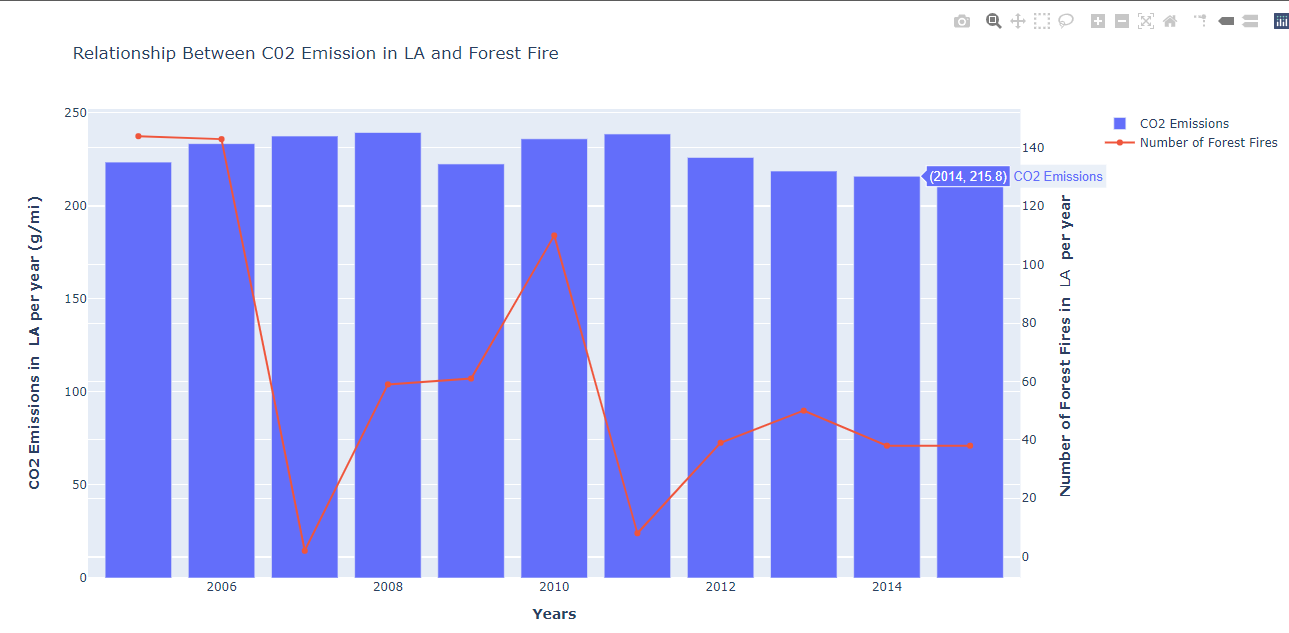
\includegraphics[width = 16cm ]{Untitled.png}
            \label{fig:my_label}
        \end{figure}
\newpage
        \item The function $entire\_plot$ is used for the second visualization. It displays a bar and line graph representing the total number of forest fires in the US in comparison to the total CO2 emissions of the US per year (this function does not have any required parameters). \\
        \begin{figure}[h]
            \centering
            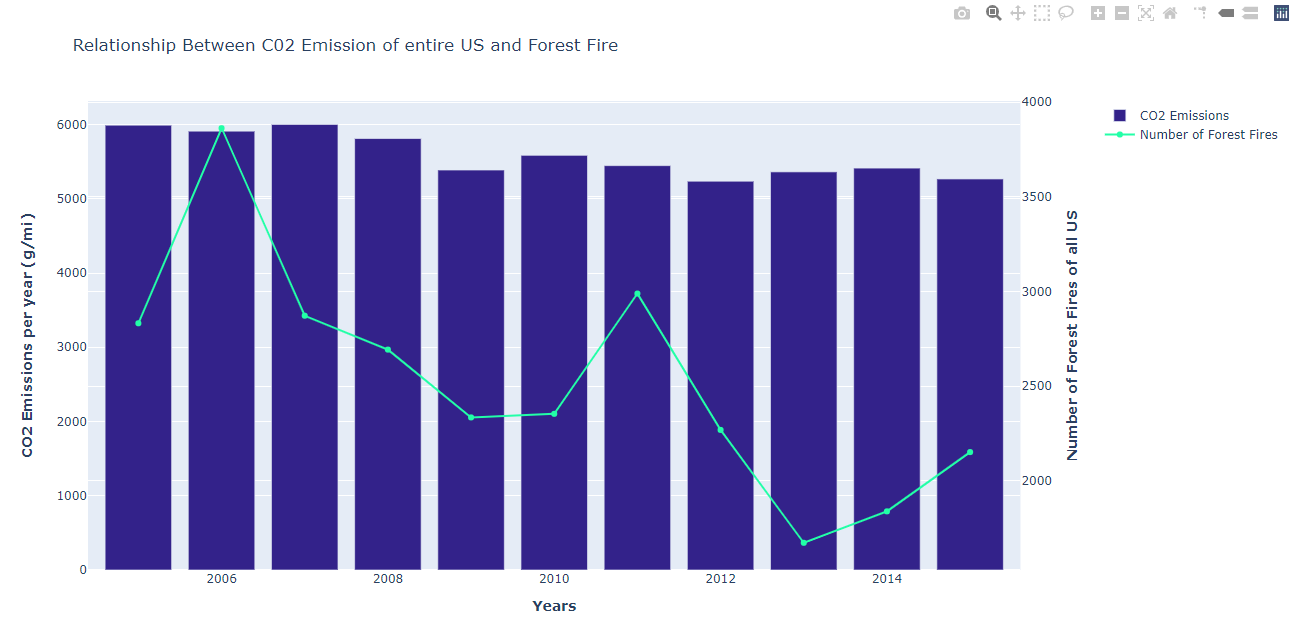
\includegraphics[width = 16cm]{usa.png}
            \label{Figure 6}
        \end{figure}
        
        \item The function $check\_trend$ requires the user to pass a state abbreviation as a parameter. The last two functions, $check\_trend$ and $check\_trend\_all$ are used to analyze the plots and determine whether or not the data proves our hypothesis. 
    \end{itemize}
    
\end{enumerate}

\section*{Instructions: Map.py}
\begin{enumerate}
    \item To begin, you need to first install the folium package 
    \item Start off by opening Pycharm and going to File$\rightarrow$ System $\rightarrow$ Project $\rightarrow$ Python Interpreter, click the add button and type $folium$ into the search bar to install the folium package. Alternatively, you can also type $pip ~ install ~ folium$ in the Pycharm terminal.
    \item Next, with the files provided through Markus, download map.py, overlay.json, requirements.txt, FireData5yrs.csv into ONE folder. For the raw FireData, check UTSend and download the data if needed (you will not need the raw data to run this file or have any functions that use the raw data)
    \item Ensure that the folder in which you store all the files in is a source root folder, do not create a sub-folder since it’s not needed.
    \item Import the libraries, check the requirements.txt file for all the libraries and their corresponding versions.
    \item Also, the overlay.json file should be left alone, it is simply used to enhance the visualization created in this file.
    \item Now that we have done all the preliminary steps, there are two 2 functions within Map.py. Note that the two functions within Map.py are called: $read\_file\_map$ and $make\_map$.
    \item $read\_file\_map$ can be called to view the processed data set, which has been formatted in the form of a Dict, where the keys represent the columns within the FireData5yrs.csv, and the values corresponding to the keys represent the data within the cells of the columns in the FireData5yrs.csv. Importantly, to call the function all the user needs to do is call the function in the console and pass “FireData5yrs.csv” as the argument to view the processed data. 
    \item However, this function is optional, it is not needed for the subsequent function to work. This is just for visualizing how the processed data looks like to have a better grasp over the wildfire data. If you do plan on running the function, USE PPRINT, it’ll be easier to view the data. 
    \item Finally, the last function remaining within the file is called $make\_map$, you can simply call it within the console, without any arguments needing to be passed within the function call. \\
    NOTE: It will take couple of seconds for the map to load, since the data is moderately large.
    \item After the function has successfully ran, you should be taken to your browser, where you should see an interactive world map, specifically zoomed to where the US is the central focus (outlined) along with other US territories.\\
    \begin{figure}[h]
            \centering
            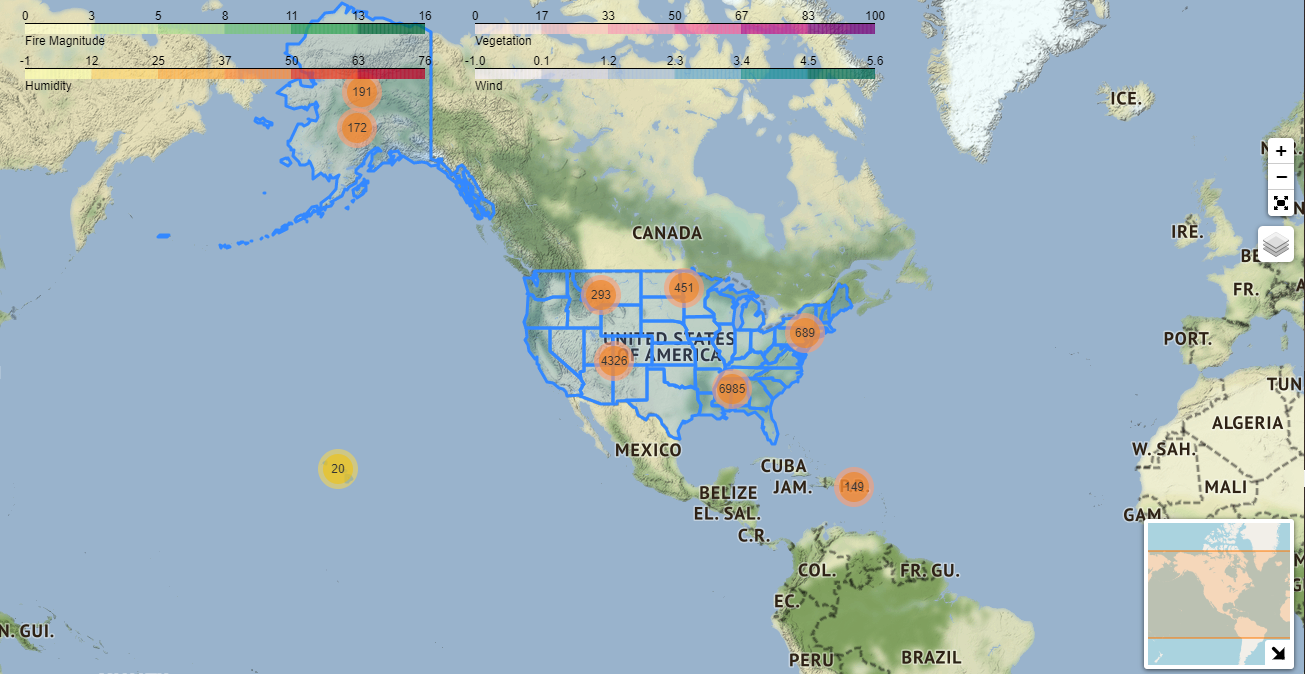
\includegraphics[width = 16cm ]{fullmapgood.png}
            \caption{Initial view of the map upon launch}
            \label{fig:my_label}
        \end{figure}
    \item Once the html file loads, the initial result should look identical to the picture provided above. The map above visualizes all of the information that was returned from the first function, $ read\_file\_map $ and specifically the (FireData5yrs.csv). Next, the map itself has a lot of features, firstly as you can see the circles on the map represent clusters of forest fires within a certain region. These dots are interactive, therefore by clicking one of the circles, it zooms in the user and the circle expands to smaller circles, which once again representing smaller clusters of forest fires.\\
    \begin{figure}[h]
            \centering
            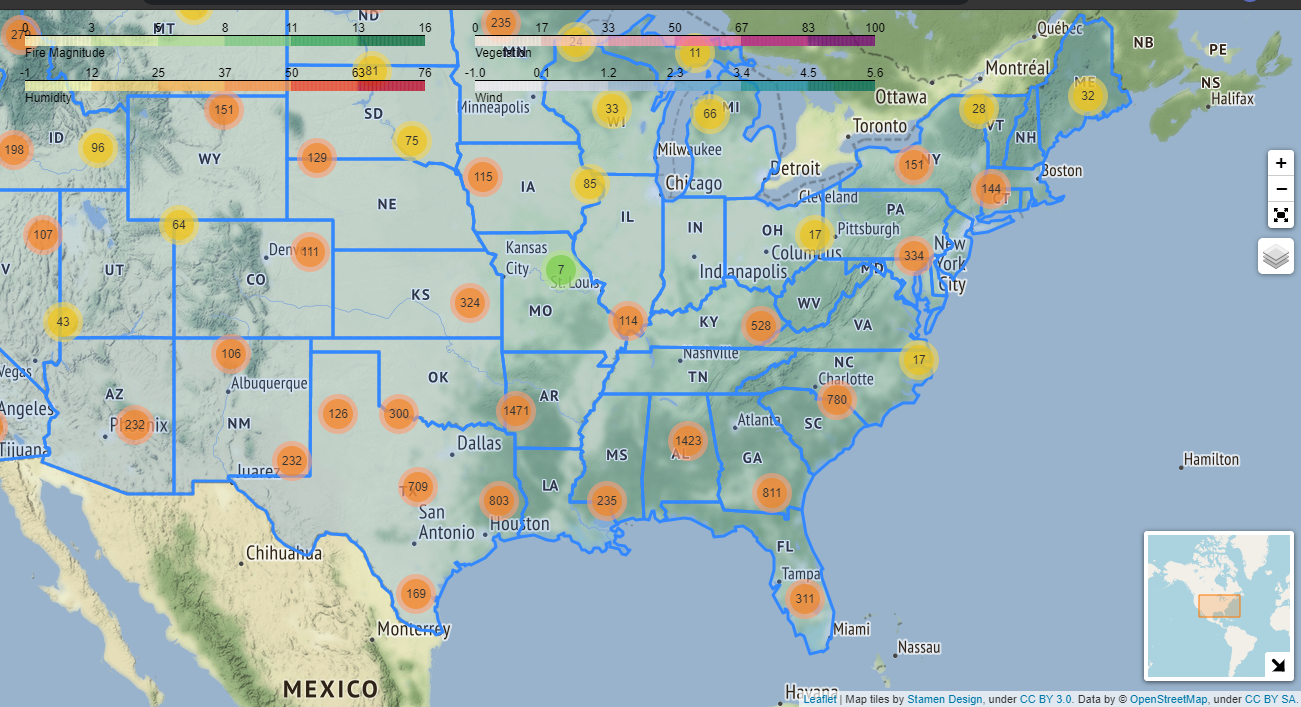
\includegraphics[width = 10cm ]{zoom1.png}
            \caption{After clicking on the 6000 Wildfire Cluster}
            \label{fig:my_label}
        \end{figure}
\newpage
    \item For example, the picture above is a result of clicking the 6985 dots(near Georgia/Alabama), which has now expanded out to other smaller dots, as you can see the number of forest fires within a cluster decreases every time you click on it. This process can be repeated until there are no more clusters of forest fires within a region but instead a specific forest fire.\\
    \begin{figure}[h]
            \centering
            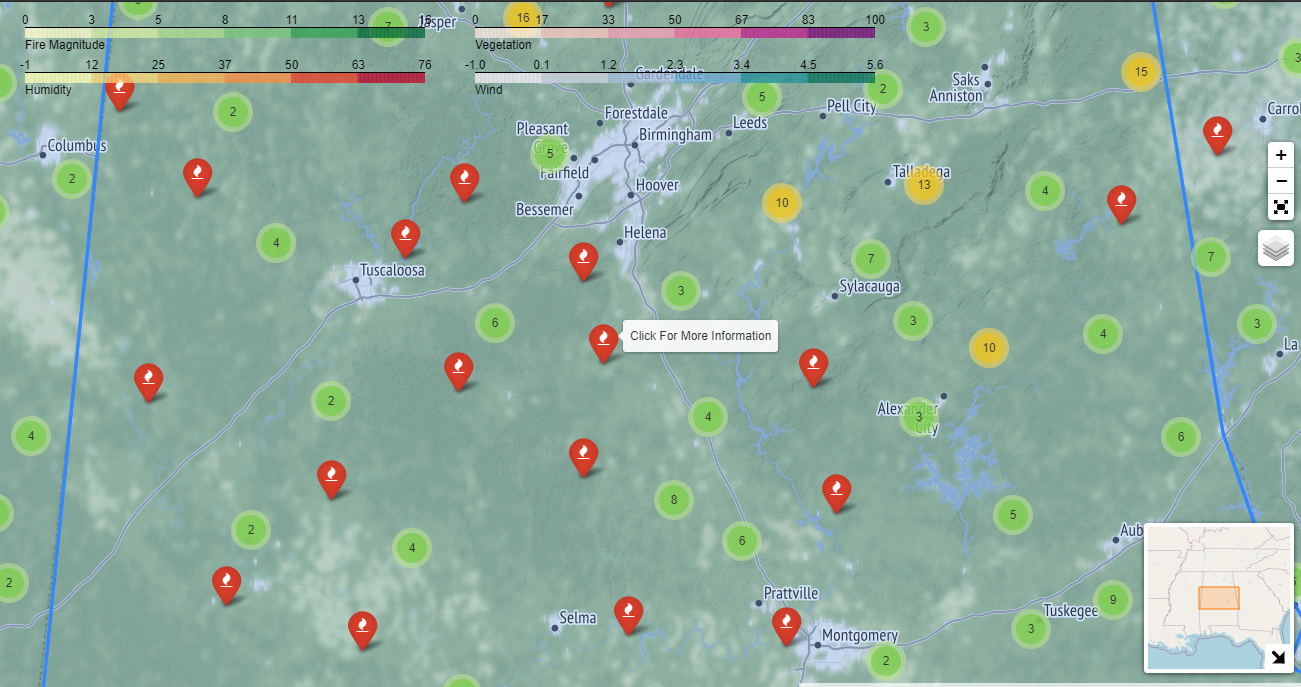
\includegraphics[width = 10cm ]{zoom2.png}
            \caption{Zooming to a Specific Wildfire and Hovering Over it}
            \label{fig:my_label}
        \end{figure}
    \item As shown above, the red fire markers represent instances of forest fires that happened at a certain location. Further, these markers are also interactive, simply by hovering over the markers we can come to know that it says “Click For More Information”. Hence, by clicking on the marker it provides informative information about the specific forest fire. Specifically, the marker popup provides insight towards fire size, fire magnitude, vegetation, wind contained, humidity contained and remoteness (check the legend for more information on the keywords). To add, a feature that was added within the popup was a hyperlink, the final line in the box relays additional information about forest fires within the state the marker is in and by clicking the link “More Details” it guides the user a link that provides that information \\
    \begin{figure}[h]
            \centering
            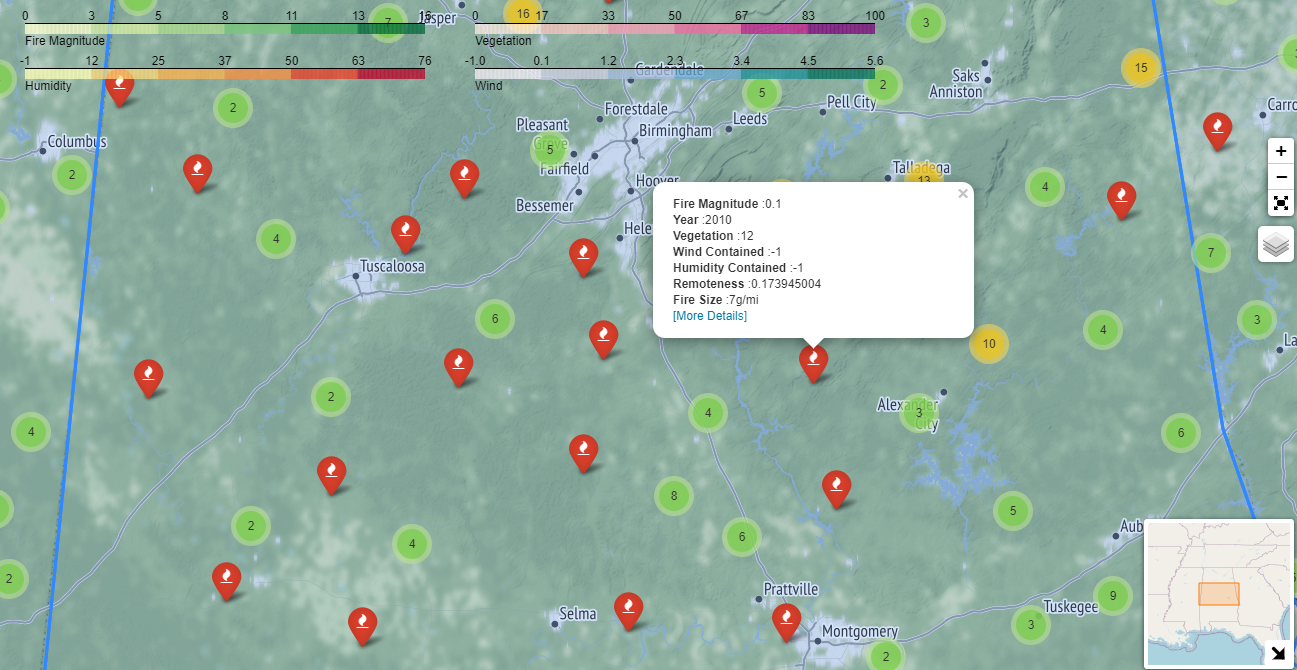
\includegraphics[width = 15cm ]{zoom3.png}
            \caption{Clicking on a Specific Wildfire Pops Open a Box}
            \label{fig:my_label}
        \end{figure}
    \item Next, as you can see in the image below, in the top right portion of your screen there are many options available. The first two options are simply for zooming in and out (also possible by scrolling your mouse). The third option is to full screen the map. Finally, the last option displayed below drops down a menu. Within the menu the user can select a type of map to their liking and finally the last options work like filters. Where if you do not want the outline of the US to be there, you can check the box off, similarly, if you do not want the marks/clusters on the map you can also turn those off. \\
    \begin{figure}[h]
            \centering
            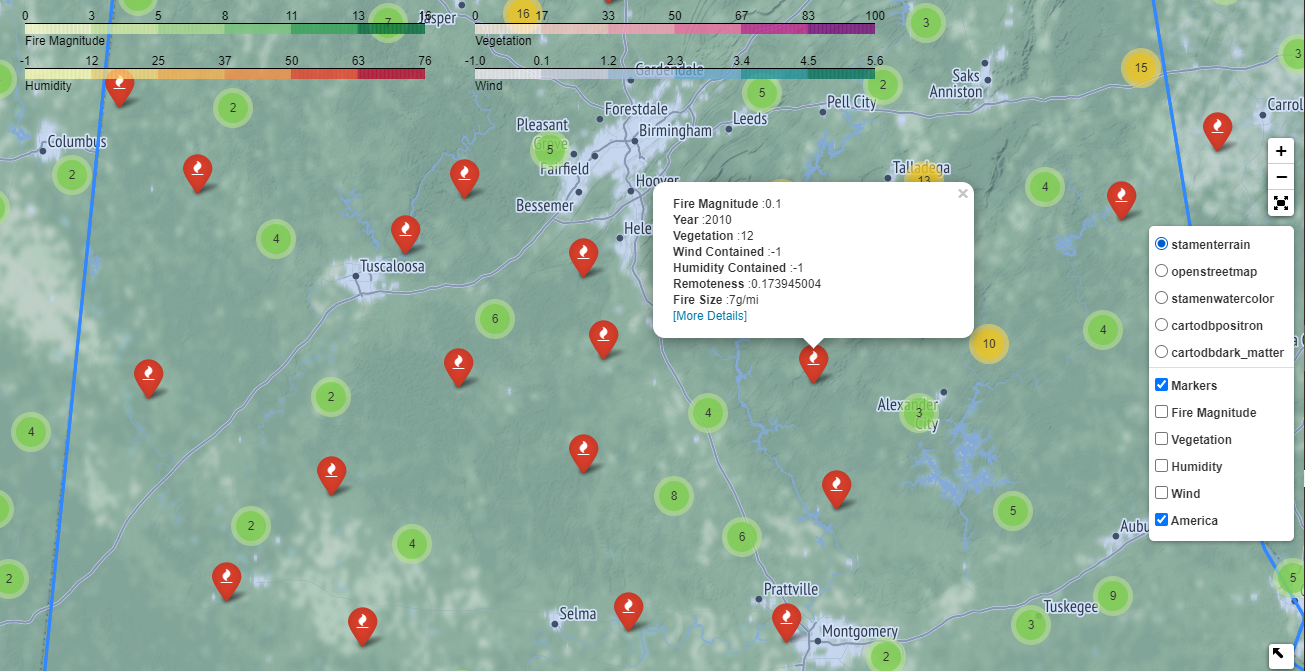
\includegraphics[width = 16cm ]{zoom4.png}
            \caption{Drop Down Menu on the Right Adds Additional Features to the Map}
            \label{fig:my_label}
        \end{figure}
    \item As an extra bonus, you can toggle the heat map on and off by filtering it with different values, like Vegetation, Fire Magnitude, Wind or Humidity. As well as a mini-map was created at the bottom which tracks your movements as you navigated through the map. It also contains a toggle which allows the user to minimize it using the diagonal arrow in the bottom right of the mini-map. \\
    \begin{figure}[h]
            \centering
            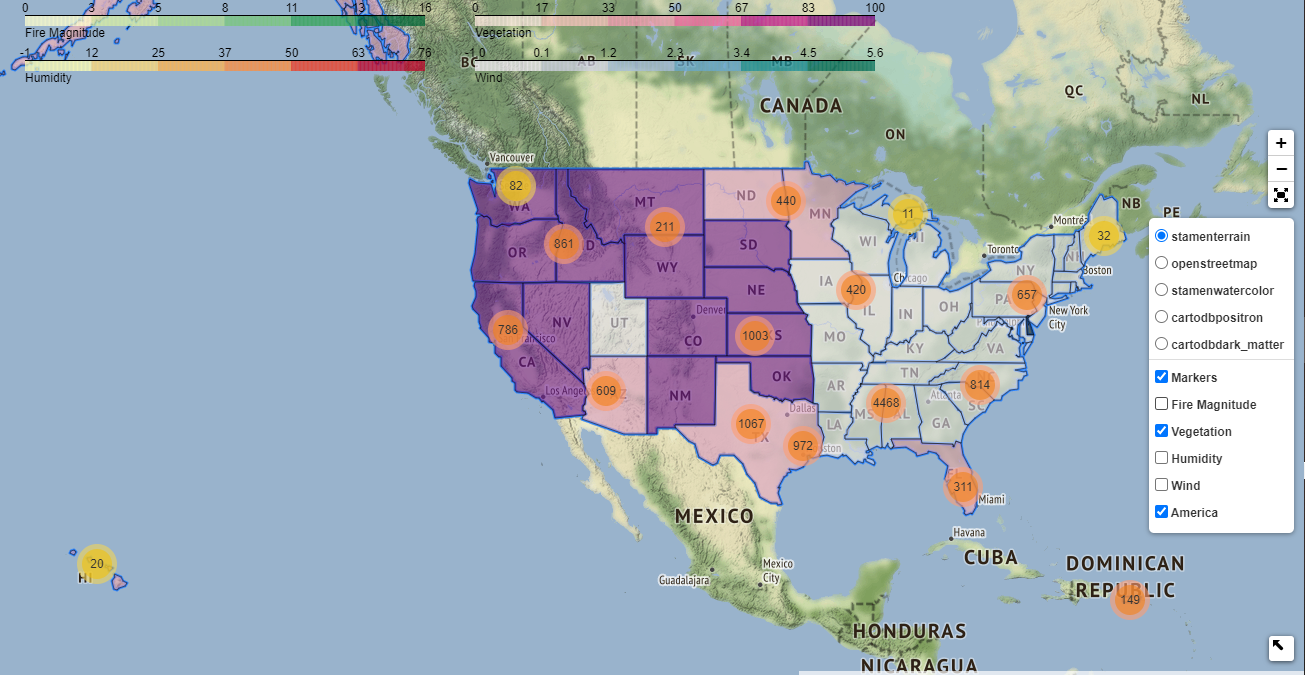
\includegraphics[width = 13cm ]{bOnus.png}
            \caption{Example a the Heat Map, filtered on Vegetation}
            \label{fig:my_label}
        \end{figure}
\end{enumerate}

\pagebreak   

\section*{Discussion Section:}
\textbf{Do the results of your computational exploration help answer this question?}
    
\begin{itemize}
\item The results of the computation did not prove our hypothesis that CO2 emissions has a correlation with forest fire frequency because through our implementation of the check\_trend\_all function and check\_trend, the visualization proves that there is little to no correlation between the CO2 levels and the number of forest fires in the US. This trend can be understood by examining the major causes of wildfires within America. Concisely, the main cause of forest fires within the US is due to human factors, a study shows “Nearly 85 percent* Wildland fires in the United States are caused by humans. Human-caused fires result from campfires left unattended, the burning of debris, equipment use and malfunctions, negligently discarded cigarettes, and intentional acts of arson” (“Wildfire Causes and Evaluations”). Therefore, the results from the visualization are valid, as CO2 levels have little to no correlation with the number of forest fires within an area. This discovery allows us to conclude that there is not a visible correlation between CO2 emissions and the frequency of forest fires in the US. This is useful for future modelling because we can now try and figure out what actually has a direct impact to forest fire frequencies.
\end{itemize}

\textbf{What limitations did you encounter with the datasets you found, the algorithms/libraries you used, or other obstacles?}
\begin{itemize}
    \item Within the study conducted, there were many instances where the shortcomings of the visualizations were due to limitations within the dataset and specific libraries chosen. First, the forest fire data set created many challenges during data wrangling. Due to the sheer size of the data (55, 000 rows), it made it challenging to filter data to our needs, specifically, due to the access number of dates, it was time-consuming to filter the years to a smaller domain. 
    \item Additionally, both datasets also contained some blank cells. This was problematic, especially with the map, as this meant that some information was missing when the markers were clicked. Therefore having to manually remove rows which contained blank cells. Additionally, the FireData10yrs.csv was not used for the simulation since the size of the file was significantly larger than the 5 year data set and would simply take too long for the html file to load. \item Next, the folium library also had many limitations. We were hoping to implement a toggle for time (years), such that if an individual were to hit the “play” button it would cycle the forest fires based on the years. However, that was not possible with the package since the toggle is only available for heat maps, which did not fit the design we were hoping to achieve. Additionally, we wanted to implement hyperlinks within the marker pop-ups, thus through extensive research, we came to know that no method/call within folium would allow us to create hyperlinks, thus we had to end up implementing the hyperlinks using HTML (language), which was tedious since it required extra research for the implementation.
    \item Furthermore, there was a major issue with the “level of detail” in the map, we hoped to have the markers decrease when zooming out and increase when we zoomed in. This task was essential due to the sheer size of the data and to prevent lag and increase usability of the map. This was originally intended to be an easy task as the leaflet (interactive JavaScript library for maps) contained a simple function .getZoom(), which would allow us to implement our intended idea. However, the same function or something similar to that was not part of folium, therefore, reading through the folium documentation, we were able to find something similar to getZoom() that implemented clusters of markers instead.
    \item Moreover, some obstacles that we faced when trying to create the graph visualizations was when we were trying to plot our original csv file that contained information of the CO2 emissions for cars and trucks we realized that the data was inaccurate and did not contain the information we needed. To remedy this, we found a new, reliable data set that represents the CO2 emissions for each state per year and plotted that information to draw our final conclusion. 
\end{itemize}
\textbf{What are some next steps for further exploration?}
\begin{itemize}
    \item Some next steps we can take to further explore our problem domain is to find a dataset that covers forest fires and CO2 emissions from 2021. We can also try and analyze data for other countries and compare the results in order to verify if the conclusion we drew form the results were accurate and come up with the actual reasoning behind why certain countries may have higher or lower amounts of forest fire. Potentially, we can expand the domain of the question from CO2 emissions to other sorts of greenhouse gasses and substances that can affect the frequency of forest fires. As mentioned before, we can do this globally or even for specific countries. The goal would remain the same where we are interested in observing the relationship between the predictor (different greenhouse gasses and response variables (forest fires)). Additionally, we believe that it would be insightful to study human behaviors to have a better understanding of forest fires. Since most forest fires are due to humans, whether that is due to cigarettes, intentional fires, or camping (not at a campsite). Overall, it would be interesting to observe the relationship between human behaviorisms, or lack thereof, and its implication on the environment and forest fires.
\end{itemize}
\hline



\newpage
\begin{center}
    {Works Cited}
\end{center}
\newline
\newline
% NOTE: LaTeX does have a built-in way of generating references automatically,
% but it's a bit tricky to use so we STRONGLY recommend writing your references
% manually, using a standard academic format like APA or MLA.
% (E.g., https://owl.purdue.edu/owl/research_and_citation/apa_style/apa_formatting_and_style_guide/general_format.html)

\noindent“Average Monthly Temperature: NOAA Climate.gov.” www.climate.gov/maps-data/data-snapshots/data-source-average-monthly-temperature. 
\newline
\newline
“Bar Charts.” Plotly, plotly.com/python/bar-charts/. 
\newline
\newline
Frohlich, Thomas C., and Liz Blossom. "These Countries Produce the Most CO2 Emissions." 14 July 2019. Web. 13 Dec. 2020. 
\newline
\newline
“Folium — Folium 0.11.0 Documentation.” Python Visualization, 2020, python-visualization.github.io/folium. 
\newline
\newline
Gray, Ellen. “Satellite Data Record Shows Climate Change's Impact on Fires – Climate Change: Vital Signs of the Planet.” NASA, NASA, 11 Sept. 2019, climate.nasa.gov/news/2912/satellite-data-record-shows-climate-changes-impact-on-fire/. 
\newline
\newline
 “Line Charts.” Plotly, plotly.com/python/line-charts/. 
\newline
\newline
Multiple Axes. (2020). Python | Plotly. https://plotly.com/python/multiple-axes/
\newline
\newline
Osmanski, Stephanie. “How Do Carbon Emissions Affect the Environment?” Green Matters, Green Matters, 30 Mar. 2020, www.greenmatters.com/p/how-do-carbon-emissions-affect-environment. 
\newline
\newline
The source of the coordinates data is from the following website : www.geojson.io
\newline
\newline
State Carbon Dioxide Emissions Data - U.S. Energy Information Administration (EIA). \\ www.eia.gov/environment/emissions/state/. 
\newline
\newline
“U.S. Wildfire Data (plus Other Attributes).” Kaggle, 6 Oct. 2020, www.kaggle.com/capcloudcoder/us-wildfire-data-plus-other-attributes.
\newline
\newline
“Wildfire Causes and Evaluations.” U.S. National Park Service, www.nps.gov/articles/wildfire-causes-and-evaluation.htm. 
\newpage
\subsection*{Extra links used just to display on the map for each state}
\newline
https://www.reuters.com/article/idUSKCN0R203U20150902?edition-redirect=ca
\newline
Scatter Plots. plotly.com/python/line-and-scatter/.
\newline
https://www.scemd.org/prepare/types-of-disasters/wildfires/#:~:text=The%20largest%20wildfire%20ever%20to,when%2014%2C405%20fires%20were%20reported.
\newline
https://en.wikipedia.org/wiki/Bastrop\_County\_Complex\_Fire#:~:text=The%20Bastrop%20County%20Complex%20fire,in%20September%20and%20October%202011.
\newline
https://www.courier-journal.com/story/news/local/2016/11/15/27-wildfires-remain-southeastern-kentucky/93913974/
\newline
https://en.wikipedia.org/wiki/1998\_Florida\_wildfires
\newline
https://abc3340.com/news/local/more-than-350-wildfires-in-september-as-alabama-is-under-a-statewide-fire-alert
\newline
https://www.audubon.org/news/alaskas-big-fire-seasons-are-new-normal-and-reshaping-landscape#:~:text=The%202004%20fire%20season%2C%20Alaska's,more%20than%206.6%20million%20acres.
\newline
https://talkbusiness.net/2018/01/arkansas-has-its-highest-wildfire-numbers-in-five-years-during-2017/#:~:text=In%202017%2C%201%2C566%20wildfires%20burned,2%2C148%20wildfires%20burned%2034%2C434%20acres.
\newline
https://www.knoxnews.com/story/news/local/tennessee/2016/12/11/how-bad-2016-fire-season/95217380/
\newline
https://www.wtnh.com/news/largest-brush-fire-in-recent-connecticut-history-burns-in-cornwall/
\newline
https://earthobservatory.nasa.gov/images/51670/fire-in-great-dismal-swamp-virginia#:~:text=Land%20Fires-,Fire%20in%20southern%20Virginia,Swamp%20on%20August%204%2C%202011
\newline
https://www.insurancejournal.com/news/southcentral/2019/08/20/536644.htm
\newline
https://en.wikipedia.org/wiki/Bugaboo\_Scrub\_Fire#:~:text=The%20Bugaboo%20Fire%20was%20a,of%20both%20Georgia%20and%20Florida.
\newline
https://en.wikipedia.org/wiki/Great\_Baltimore\_Fire#:~:text=The%20Great%20Baltimore%20Fire%20raged,to%20an%20estimated%20%24100%20million.
\newline
https://en.wikipedia.org/wiki/Great\_Fire\_of\_New\_York#:~:text=The%201835%20Great%20Fire%20of,the%2018th%20and%2019th%20centuries.
\newline
https://en.wikipedia.org/wiki/Great\_Michigan\_Fire
\newline
https://mrcc.illinois.edu/living\_wx/wildfires/index.html#:~:text=The%20Great%20Chicago%20Fire%20that,of%20up%20to%20300%20people.
\newline
https://idahonews.com/sponsored/spotlight/important-facts-about-major-wildfires-in-idaho-history#:~:text=The%20Murphy%20Complex%20Fire%20in,southern%20Idaho%20and%20northern%20Nevada.
\newline
https://wildfiretoday.com/tag/jasper-fire/
\newline
https://www.kansascitymag.com/kansas-now-has-a-wildfire-season-heres-what-that-means/#:~:text=In%20March%202016%2C%20the%20Anderson,largest%20fire%20in%20Kansas%20history.
\newline
https://www.clarionledger.com/story/news/2017/03/24/mississippi-wildfires/99573416/
\newline
https://en.wikipedia.org/wiki/Las\_Conchas\_Fire#:~:text=The%20Las%20Conchas%20Fire%20was,the%20town%20of%20Los%20Alamos.
\newline
https://www.areawidenews.com/story/1875438.html
\newline
https://earthobservatory.nasa.gov/images/18693/milford-flat-fire-utah#:~:text=Land%20Fires-,Milford%20Flat%20Fire%2C%20Utah,sagebrush%2C%20driven%20by%20the%20wind.
\newline
https://bringmethenews.com/minnesota-lifestyle/remembering-the-monster-wildfires-of-minnesotas-history
\newline
https://www.greatfallstribune.com/story/news/2020/10/03/montana-fires-most-destructive-wildfires-2020-bridger-foothills-bobcat-fire/5894963002/
\newline
https://en.wikipedia.org/wiki/Martin\_Fire
\newline
https://www.wbur.org/earthwhile/2020/09/15/new-hampshire-wildfire-risk-climate-change
\newline
https://en.wikipedia.org/wiki/New\_Jersey\_Forest\_Fire\_Service#:~:text=In%20two%20days%2C%20on%20April,were%20killed%20in%20the%20incident.
\newline
https://www.hawaiiwildfire.org/news-center
\newline
https://spectrumnews1.com/oh/columbus/weather/2020/10/20/wildfire-threats-in-ohio#:~:text=In%20Ohio%2C%20most%20of%20our%20wildfires%20are%20human%20influenced.&text=In%202019%2C%20there%20was%20a,total%20of%20733%20acres%20burned.
\newline
https://www.cnn.com/2020/03/08/us/oklahoma-412-fire/index.html
\newline
https://stateimpact.npr.org/pennsylvania/2016/04/27/pocono-forest-fire-destroys-more-than-8000-acres/#:~:text=The%20fire%20stretched%2016%20miles,been%20burning%20for%20a%20week.
\newline
https://history.nebraska.gov/publications/prairie-fires#:~:text=Some%20news%20accounts%20have%20alleged,the%20Great%20Plains%20in%201865.
\newline
https://en.wikipedia.org/wiki/Bastrop\_County\_Complex\_Fire#:~:text=The%20Bastrop%20County%20Complex%20fire,in%20September%20and%20October%202011.
\newline
https://www.newenglandhistoricalsociety.com/four-days-may-1942-rhode-island-forest-fires/
\newline
https://www.maine.gov/dacf/mfs/forest\_protection/1947\_fire.html#:~:text=In%201947%2C%20the%20State%20of,and%20spread%20out%20of%20control.
\newline
https://www.opb.org/news/series/wildfires/oregon-biscuit-fire-history-largest-ever/#:~:text=In%20July%20of%202002%2C%20a,forest%20fire%20in%20Oregon's%20history.&text=The%20fire%20left%20nearly%20half,finally%20fizzled%20out%20months%20later.
\newline
https://www.5280.com/2020/10/the-10-largest-wildfires-in-colorados-history/
\newline
https://en.wikipedia.org/wiki/Evans\_Road\_Wildfire#:~:text=The%20Evans%20Road%20Wildfire%20was,and%20burned%20for%20three%20months.
\newline
https://www.nps.gov/jeca/learn/nature/jasperfire.htm
\newline
https://earthobservatory.nasa.gov/images/50999/wallow-fire-arizona#:~:text=On%20June%2013%2C%20the%20Wallow,commercial%20buildings%2C%20and%2036%20outbuildings.
\newline
https://www.wgbh.org/news/local-news/2020/09/08/western-mass-blaze-serves-as-reminder-of-states-rich-history-of-wildfire
\newline
https://www.scemd.org/prepare/types-of-disasters/wildfires/#:~:text=The%20largest%20wildfire%20ever%20to,when%2014%2C405%20fires%20were%20reported.
\newline
https://www.firehouse.com/operations-training/article/10502384/wildland-fire-sweeps-iowa-countryside
\newline
https://dnr.wisconsin.gov/topic/forestfire/wisconsinfires#:~:text=Peshtigo%20Fire%20%7C%201871,estimated%20%24169%20million%20in%20damages.


\end{document}
